% !TEX encoding = UTF-8 Unicode
\documentclass[fleqn,twoside]{article}
\usepackage[ngerman]{babel}
\usepackage[utf8]{inputenc}
\usepackage[T1]{fontenc}
\usepackage{amsmath}
\usepackage{amssymb}
\usepackage{booktabs}
\usepackage{calligra}
\usepackage{cite}
\usepackage{comment}
\usepackage{csquotes}
\usepackage{enumitem}
%\usepackage{eurosym}
\usepackage{fancyhdr}
\usepackage{fdsymbol}
\usepackage{float}
\usepackage{graphicx}
\usepackage{graphicx}
\usepackage{multirow}
\usepackage{nicefrac}
\usepackage{pdfpages}
\usepackage{pifont}
\usepackage{romanbar}
\usepackage{siunitx}
\usepackage{stanli}
\usepackage{svg}
\usepackage{tabto}
\usepackage{tabularx}
\usepackage{textcomp}
\usepackage{tikz}
\usepackage{titlesec}
\usepackage{todonotes}
\usepackage{wasysym}
\usepackage{wrapfig}
\usepackage{yfonts}
\usepackage{marvosym}
%\usepackage{3dstructuralanalysis}
%\usepackage{emerald}
%\usepackage{structuralanalysis}
%\usepackage{units}



%Befehle abändern
%Itemize ohne Lücken
\setlist[itemize]{noitemsep, topsep=2pt}
\raggedbottom
%\renewcommand{\todo}[1]{\todo[inline]{#1}}


%Betragsfunktion
\newcommand{\abs}[1]{\ensuremath{\left\vert#1\right\vert}}
%Einheitenfunktion
\newcommand{\un}[2]{{\unit[#1]{\color{black!100}[#2]}}}

\usepackage[pdftex, colorlinks, linkcolor=black, frenchlinks]{hyperref}
\usepackage[a4paper , lmargin = {2.5cm} , rmargin = {2cm} , tmargin = {2.5cm} , bmargin = {2.5cm} ]{geometry}
\pagestyle{fancy}

\title{\Huge{\textfrak{Innovationen und Entwicklungen im Holzbau}}}
\author{\calligra{Jonas Konrad}}
\date{\textfrak{\today}}

\begin{document}
\parindent 0pt
\fancyhead[L]{Jonas Konrad}
\fancyfoot[L]{\frakfamily J. K.}
\fancyfoot[R]{\frakfamily }
\fancyfoot[C]{\frakfamily "Was soll man da eigentlich lernen? Wir haben ja nichts gemacht" \\Seite \thepage}
\maketitle \thispagestyle{empty}
%\initfamily %Für Initialien
\begin{center}
\textfrak{Diese Sammlung der Vorlesungsinhalte wurde im Wintersemester 2022/23 von Jonas Konrad verfasst.\\Dozent: Dr.ir. Carmen Sandhaas , Übungsleiter: M.Sc. Simon Aurand\\Kein Anspruch auf Vollständigkeit oder Fehlerfreiheit.\\LaTex Vorlage: github.com/Neowise33}
\end{center}
\tableofcontents
%\listoftodos
\newpage

%\listoftodos
%\newpage



\section{Einführung}

\subsection{Bereiche der Innovation und Entwicklung}
    \begin{itemize}
        \item Baustoffe: z.B. Baubuche
        \item Verbindungen: z.B. Klebetechniken
        \item Tragwerke: z.B. Autobahnbrücke aus blockverklebte vorgespannte Akoya
    \end{itemize}

\subsection{Ziele des modernen Holzbaus}
    \begin{itemize}
        \item höher als vor einige Jahren
        \item mit unterschiedlichen Materialien
        \item mit flächigen Bauteilen
    \end{itemize}

\subsection{Entwurf und Bemessung:}
    Tragwerk benötigt Symbiose aus:
    \begin{itemize}
        \item mechanischem Verständnis
        \item Materialkenntnisse
        \item gutem Konstruieren
    \end{itemize}

\subsection{Technische Regelungen: Baurecht}
    \subsubsection{Rechtliche Grundlagen:}
    \begin{itemize}
        \item Eurocode
        \item ETA (Europäische Technische Bewertung $\rightarrow$ CE-Zeichen, Leistungserkärung des Herstellers)
        \item (DIN-)Normen
        \item Nationale Regelungen (abZ, aBG, ZiE, vBG):
        \end{itemize}
            \hspace*{5mm} $\begin{aligned}&\left.
            \begin{array}{l}
                \text { - Allgemeine bauaufsichtliche Zulassung (abZ) } \\
                \text { - Allgemeine Bauartgenehmigung (aBG) }
            \end{array}\right\} 
                \begin{array}{l}
                \text { ETA für DE} 
                \end{array}
            \end{aligned}$
            
            \hspace*{5mm} $\begin{aligned}&\left.
                \begin{array}{l}
                    \text { - Zustimmung im Einzelfall (ZiE) } \\
                    \text { - vorhabenbezogene Bauartgenehmigung (vBG) }    
                \end{array}\right\} \text { Schnell neues umsetzen }
            \end{aligned}$

    \begin{itemize}
        \item Landesrecht: LBO Baden-Wuerttemberg
        \item Bauproduktverordnung
        \item Baurechtliches Basiswissen: DIBt.de
    \end{itemize}
        Beispiele DIN-Normen:
        \begin{itemize}
            \item Beispiel 1\\
                DIN EN 14081-1: „Bauholz mit rechteckigem Querschnitt“
                Aufbau der Norm:
                \begin{itemize}
                    \item Teile 1 bis 3
                    \item „Unternormen“, die z.B. die mechanischen Kennwerte festlegen $\rightarrow$ EN 338
                \end{itemize}
            \item Beispiel 2\\
                DIN EN 14080: „Brettschichtholz und Balkenschichtholz“ \\ 
                $\rightarrow$ neue Generation europäischer Normen mit wenigen Unternormen
        \end{itemize}
        \begin{itemize}
            \item Anhang ZA: Legt Bedingungen für die CE-Kennzeichnungen fest
        \end{itemize}
    
    \subsubsection{CE-Kennzeichen}
        \begin{itemize}
            \item Aufpassen: CE-Kennzeichnung ist rechtlich gesehen KEIN Gütesiegel!\\
            Es wird mit der Kennzeichnung lediglich die Konformität mit bestehenden Produktrichtlinien gewährleistet\\
            $\rightarrow$ CE ist Handelszeichen für den freien Warenaustausch
        \end{itemize}
    
    \subsubsection{Systeme der Konformitätsbescheinigungen}
        \begin{minipage}{0.5\textwidth}
            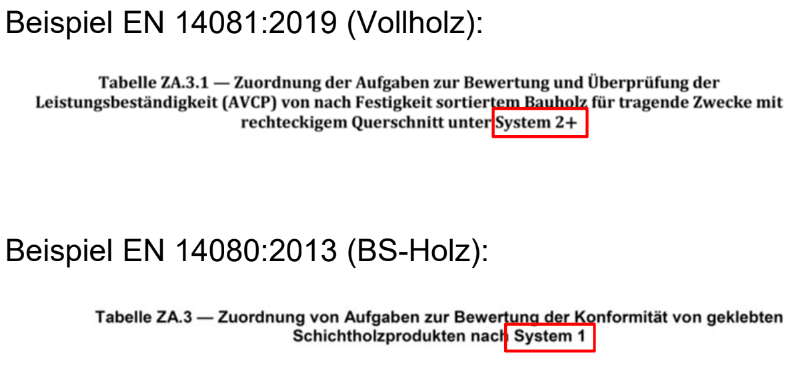
\includegraphics[width=0.9\textwidth]{Grafiken/Einführung/Konformitaetsbesch. Bsp.png}
        \end{minipage}
        \begin{minipage}{0.5\textwidth}
            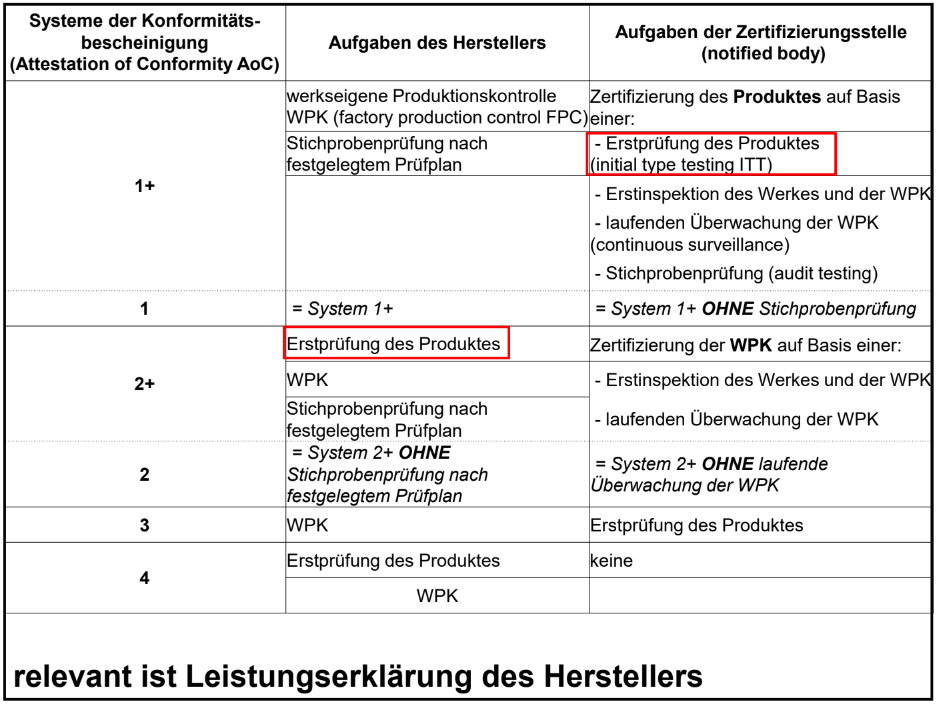
\includegraphics[width=0.9\textwidth]{Grafiken/Einführung/Konformitaetsbesch. Tabelle.png}
        \end{minipage}

    \subsection{Wie sieht es in der Praxis aus?}
        \begin{itemize}
            \item $\rightarrow$ Tabellenwerke von Herstellern
            \item \enquote{Normen ersetzen keine Erfahrung}
            \item Auspassen mit verschiedenen Normen, ETAs und Zulassungen!
                \begin{itemize}
                    \item Beispiel Bestimmung Ausziehtragfähigkeit:\\
                        $\begin{gathered}
                        F_{w, k}=f_{w, k} \cdot \pi \cdot d \cdot L_{\text {ef }} \\
                        f_{a x}=\frac{F_{a x}}{d \cdot L_{e f}} \overset{\text{\Lightning}}{\Longleftrightarrow} F_{a x}=f_{a x} \cdot \pi \cdot d \cdot L_{e f}
                        \end{gathered}$\\
                        Gleiche Variable in verschiedenen Normen, \\
                        aber unterschiedliche Berechnungsweisen und somit statische Bedeutungen
                    \item Festigkeitsklassen Vollholz aus Nadelholz:\\
                        EN 338:2003: $\mathrm{C} 24 \mathrm{f}_{\mathrm{v}, \mathrm{k}}=2,5 \mathrm{MPa}$\\
                        EN 338:2016: $\mathrm{C} 24 \mathrm{f}_{\mathrm{v}, \mathrm{k}}=4,0 \mathrm{MPa}$\\
                        EN 1995-1-1:2010, Abschnitt 6.1.7 Schub: $\tau_d \leq f_{v, d}$\\
                        $\mathrm{f}_{\mathrm{v}, \mathrm{d}}$ wird ermittelt mit $\mathrm{b}_{\mathrm{ef}}=\mathrm{k}_{\mathrm{cr}} \cdot \mathrm{b}$\\
                        und $\mathrm{k}_{\mathrm{cr}}=0,67$ für Vollholz (aufgrund von Schwindrissen)
                \end{itemize}
        \end{itemize}


        
\newpage
\section{CLT – Verbindungen}

Vorlesungsfolien lesen!\vspace{3mm}

Was gibt es generell für Verbindungen:
    \begin{itemize}
        \item Zuganker
        \item Winkel Ableitung Horizontalkraft
        \item CLT-Wandstöße über Sperrholz oder Hartholzbretter verschrauben / über flachen Blattstoß verschrauben
        \item Deckenstoße mit übergreifenden selbstbohrenden Schrauben verbinden 
        \item shear keys aus (Buchen-)Hartholz
    \end{itemize}

Generelle Verbindungsstellen:
    \begin{itemize}
        \item Verbindungen in Bauteilebene
        \item Eckverbindungen
            \begin{itemize}
                \item Von außen verschraubt (Gefahr Hirnholzverschraubung)
                \item Von innen verschraubt
                \item Von innen mit Metallwinkel verschraubt
            \end{itemize}
        \item Wand - Decke Verbindungen\\
            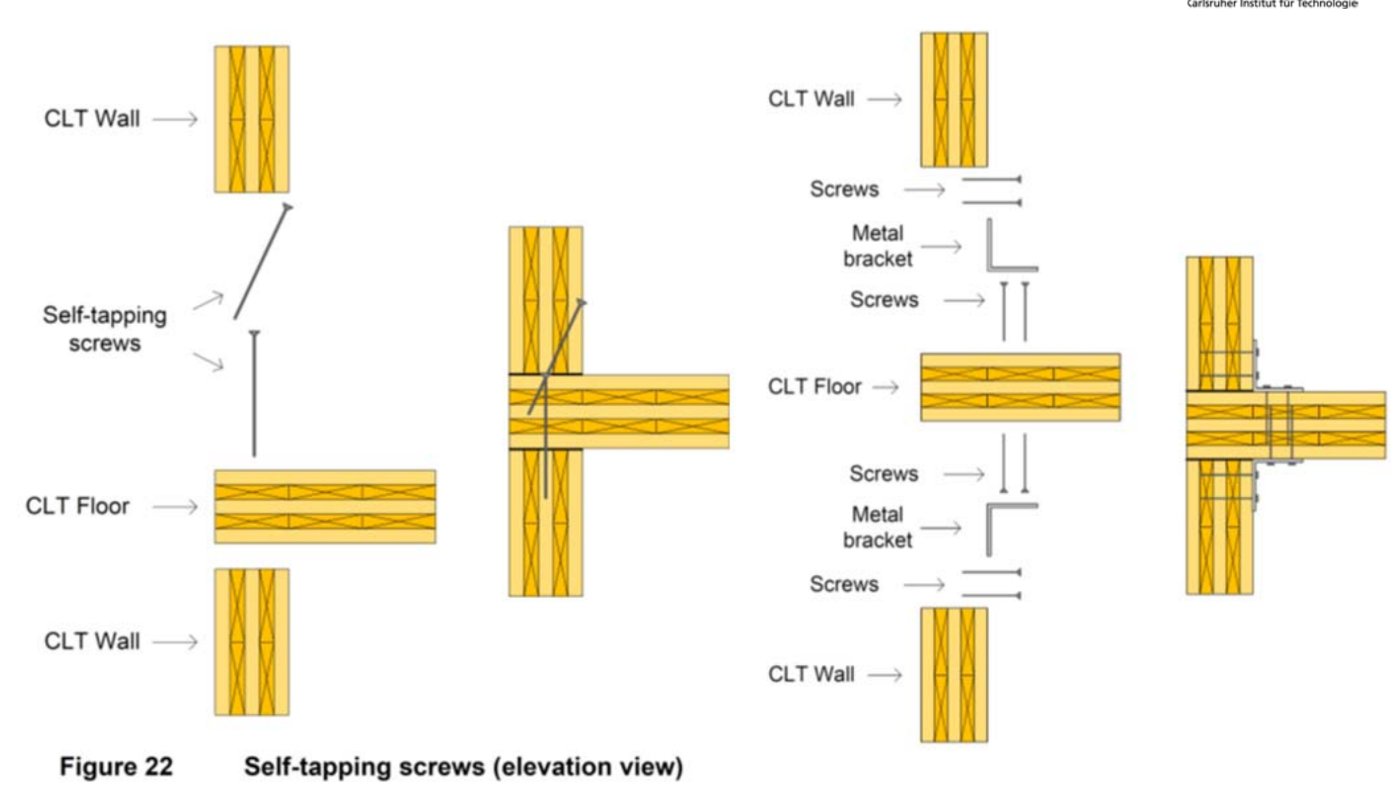
\includegraphics[width=0.45\textwidth]{Grafiken/CLT-Verbindungen/Wand-Decke mit Schrauben.png}
            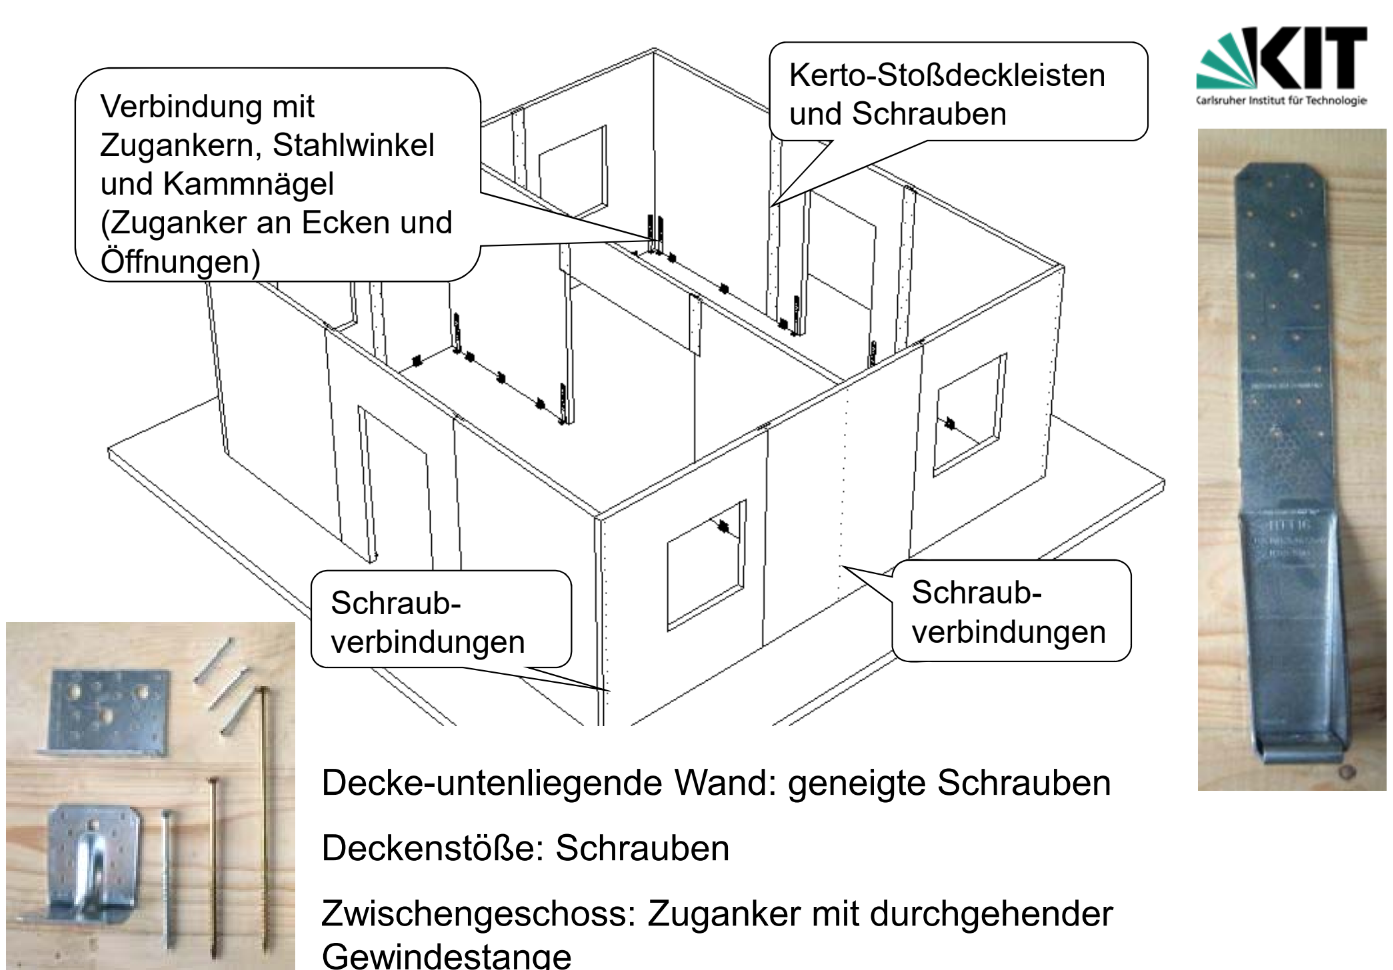
\includegraphics[width=0.45\textwidth]{Grafiken/CLT-Verbindungen/Wand-Decke Uebersicht.png}\\
            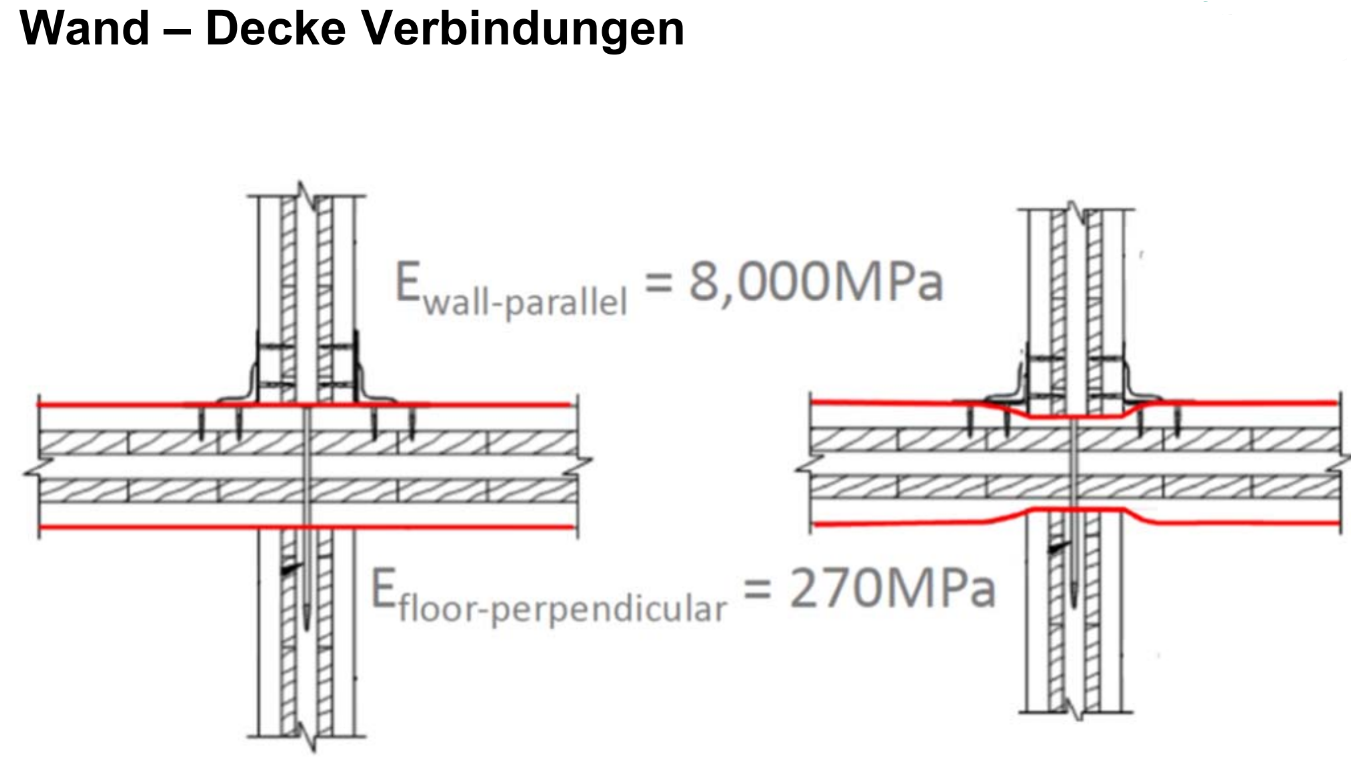
\includegraphics[width=0.45\textwidth]{Grafiken/CLT-Verbindungen/Wand-Decke Pressung.png}
            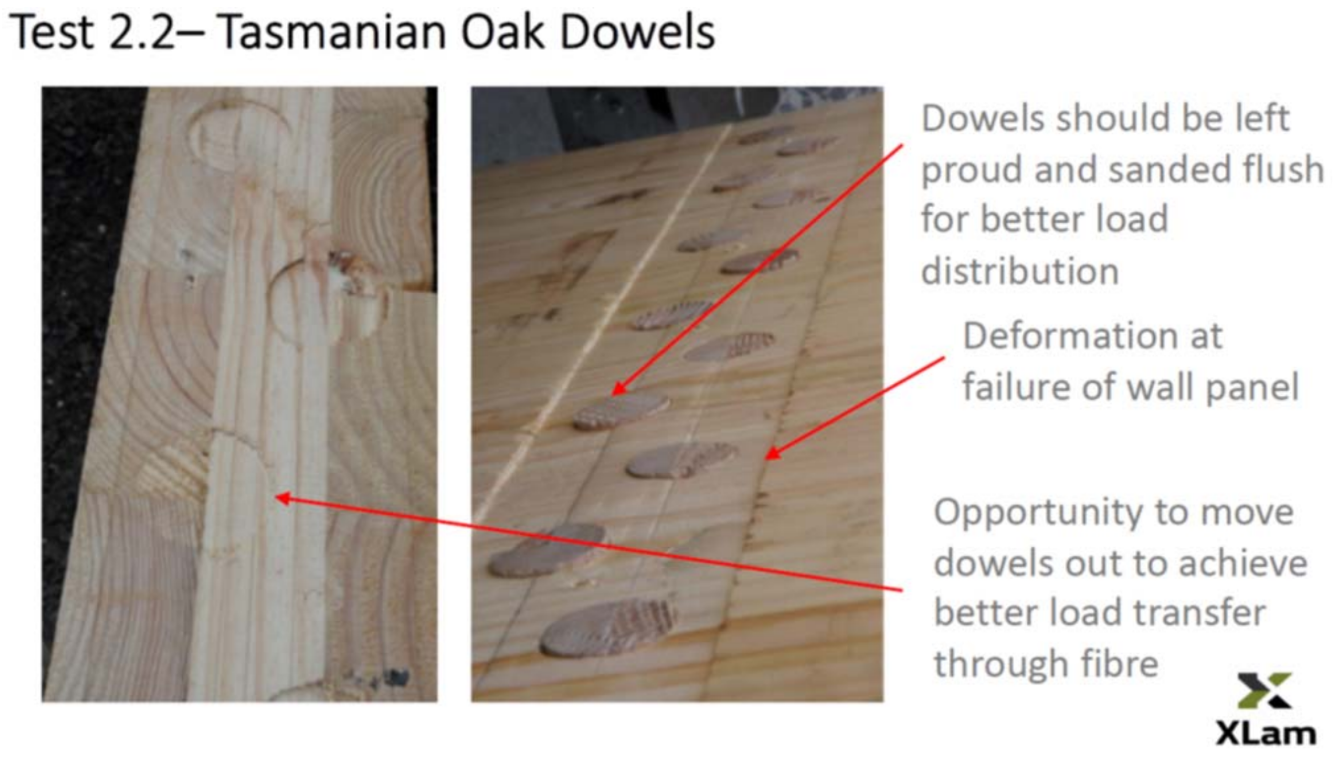
\includegraphics[width=0.45\textwidth]{Grafiken/CLT-Verbindungen/Wand-Decke Dowels.png}\\
            Weitere Dübelarten: Beton, Buchenfurnierschichtholz, eingeschraubte Metallplatten (nicht so gut)\\
            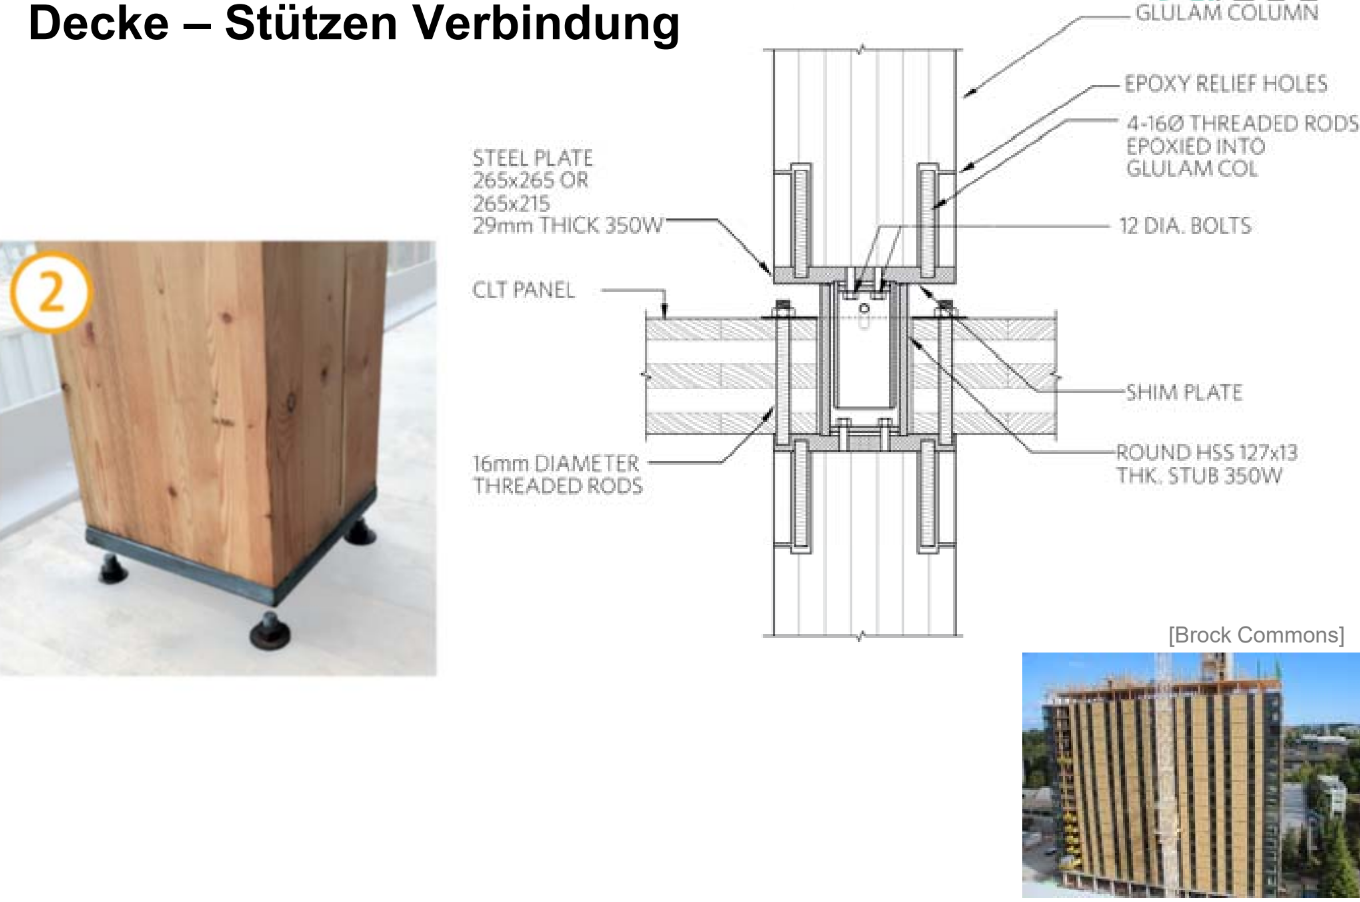
\includegraphics[width=0.45\textwidth]{Grafiken/CLT-Verbindungen/Wand-Decke Pressung Sonerloesung.png}
            
        \item Wand - Dach Verbindungen
            \begin{itemize}
                \item Geneigte Winkel entlang der Dachfußpunkte
            \end{itemize}
        \item Wand - Bodenplatte Verbindungen
            \begin{itemize}
                \item Zuganker
                \item Winkel (in BP verdübelt)
                \item Schlitzbleche auf Fundament aufgebracht und mit selbstbohrenden Stabdübeln mit CLT verbunden
            \end{itemize}
    \end{itemize}

Speziellere Verbindungen:
    \begin{itemize}
        \item CLT auf Zug eingebrachte Bolzen die in Dose zwischen Träger mit Muttern angeschraubt werden (Nachspannbarkeit, Lösbarkeit)\\
        
    \end{itemize}

Besonderheiten CLT:
    \begin{itemize}
        \item Im Vergleich zu Holztafelbau sehr steif $\rightarrow$ Kippt eher als dass es sich verformt, dadurch sehr konzentrierte Last auf Schubverbindungen zwischen Tafelelementen\\
        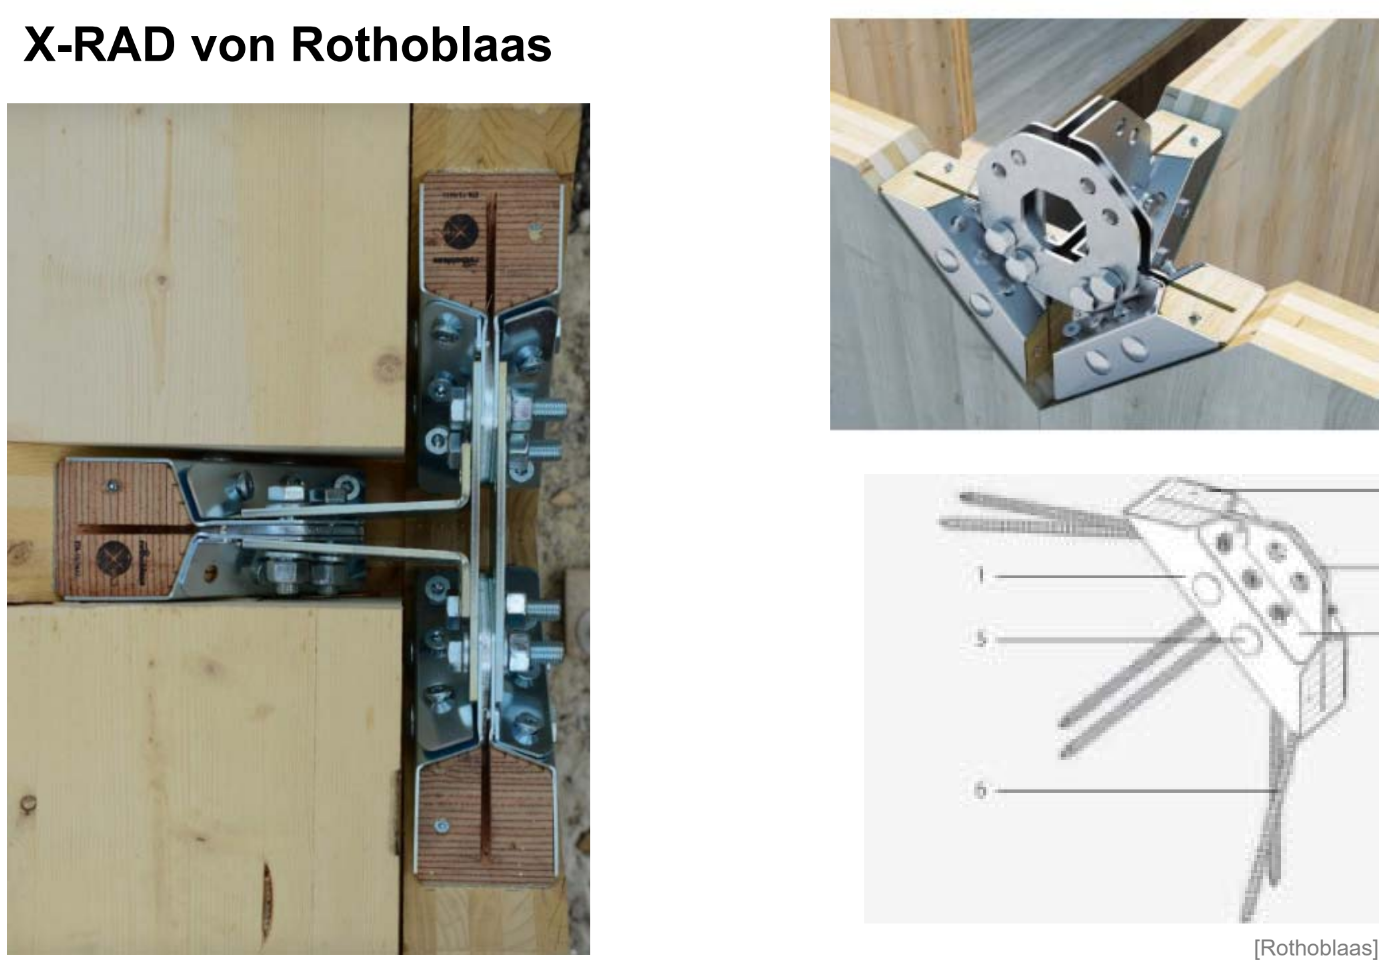
\includegraphics[width=0.45\textwidth]{Grafiken/CLT-Verbindungen/X-RAD Rothoblaas.png}
        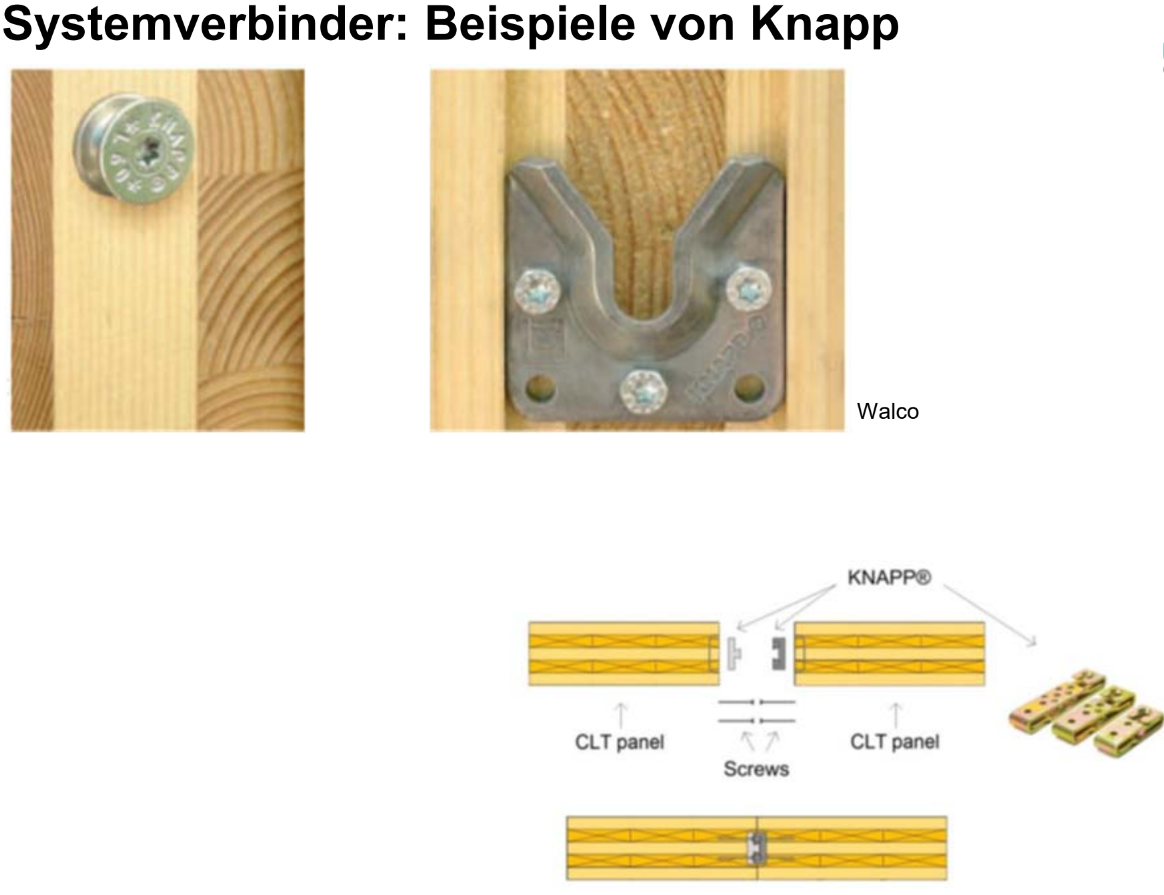
\includegraphics[width=0.45\textwidth]{Grafiken/CLT-Verbindungen/Knapp Systemverbinder.png}\\
        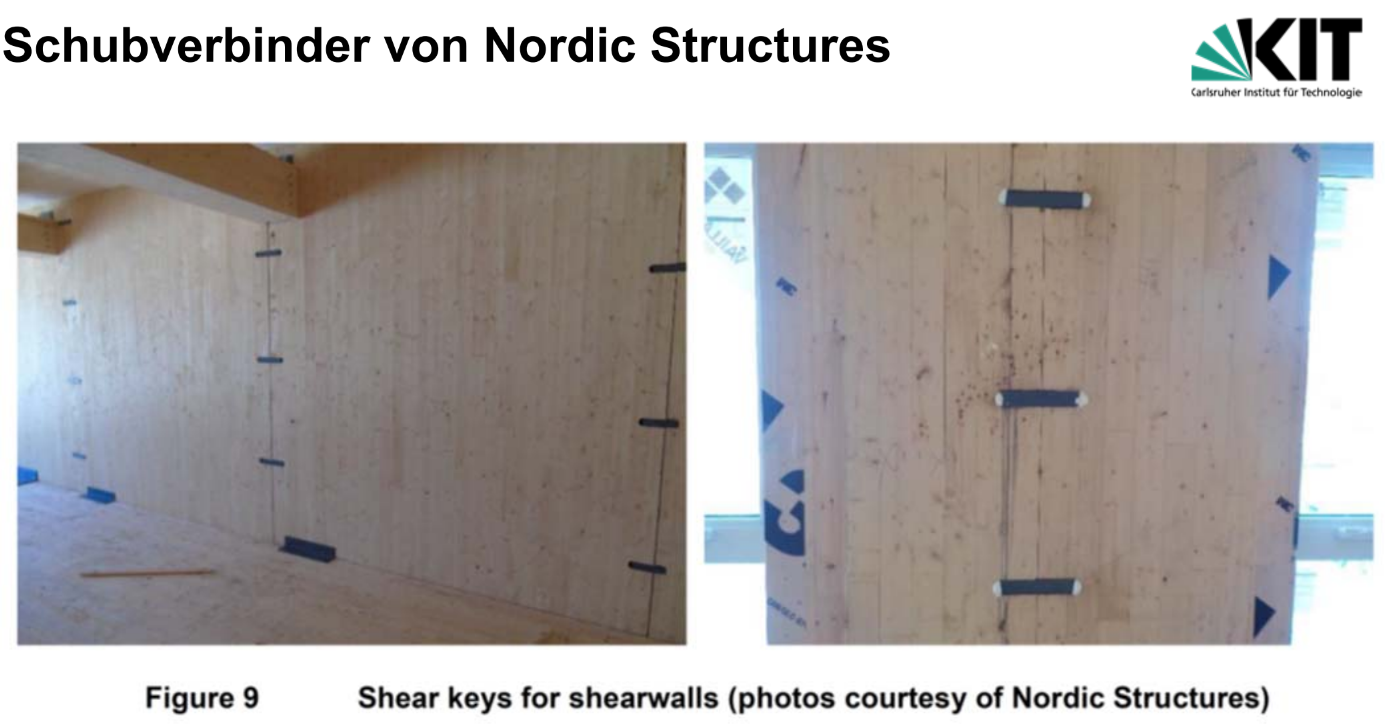
\includegraphics[width=0.45\textwidth]{Grafiken/CLT-Verbindungen/Nordic Structures Schubverbinder.png}
        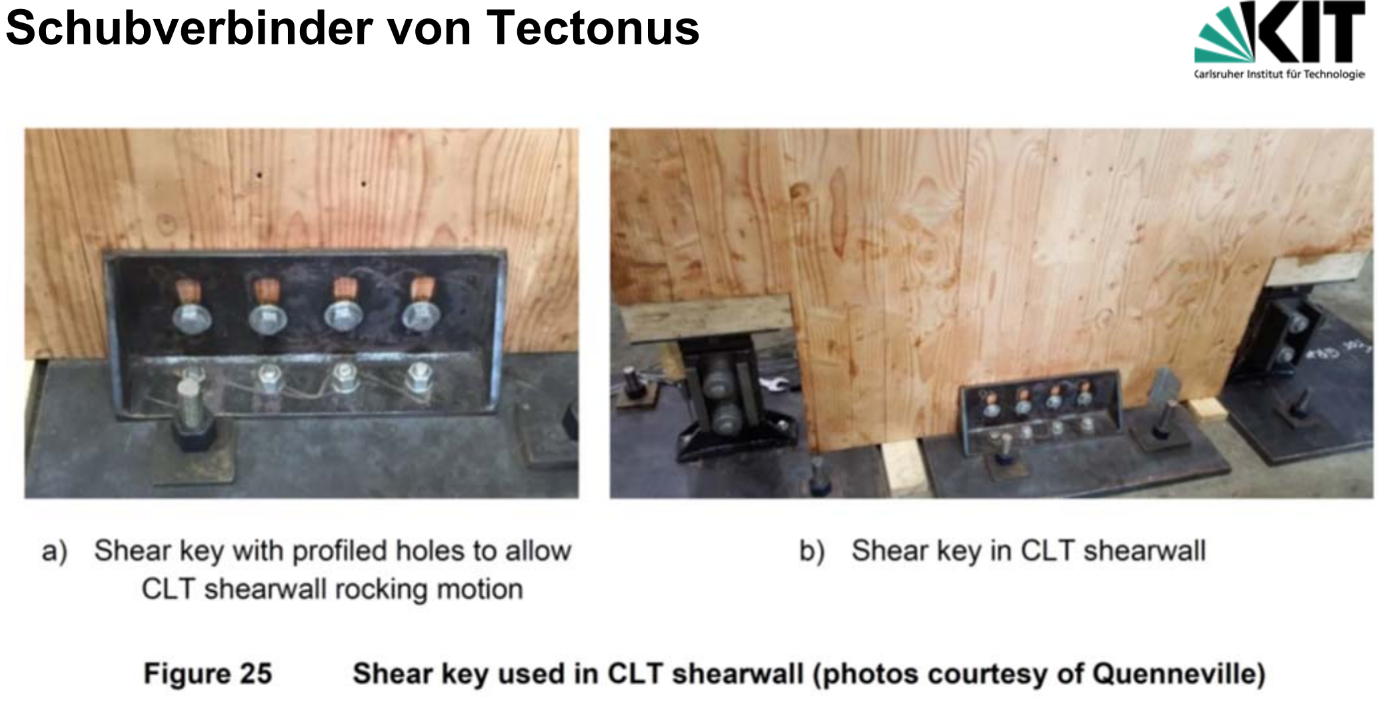
\includegraphics[width=0.45\textwidth]{Grafiken/CLT-Verbindungen/Tectonus Schubverbinder.png}\\
        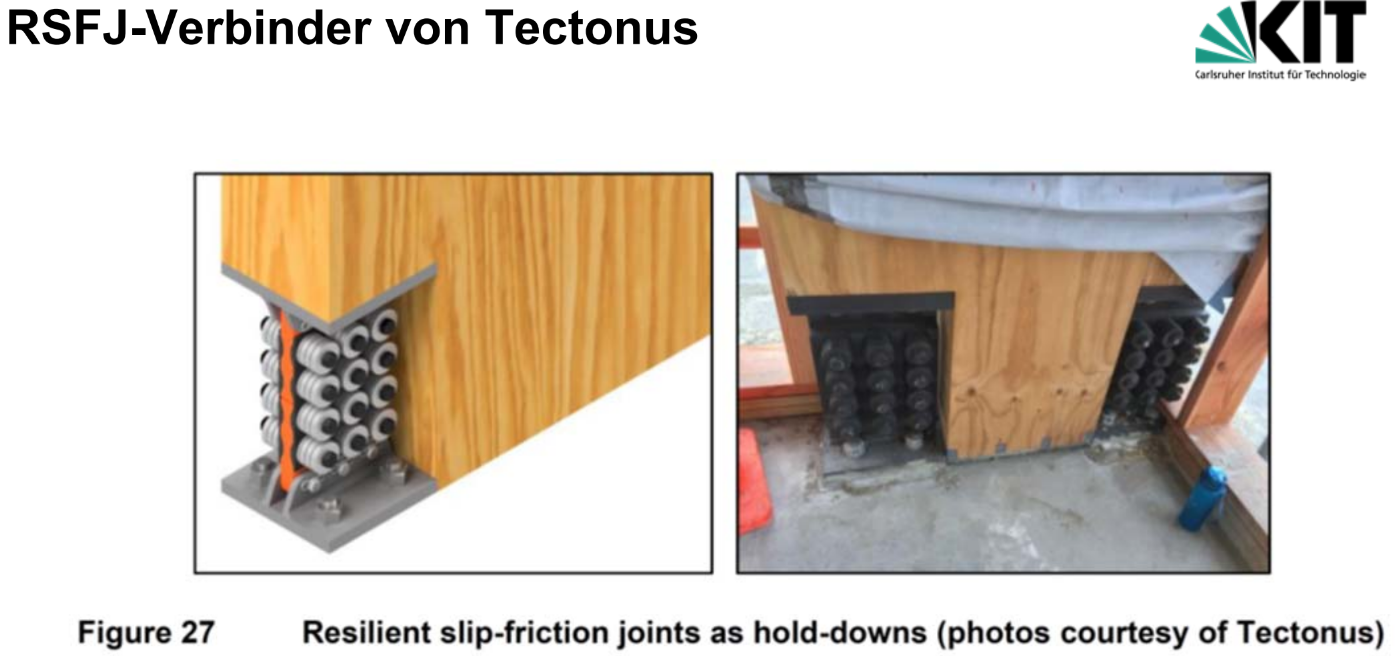
\includegraphics[width=0.45\textwidth]{Grafiken/CLT-Verbindungen/Tectonus RSFJ.png}
        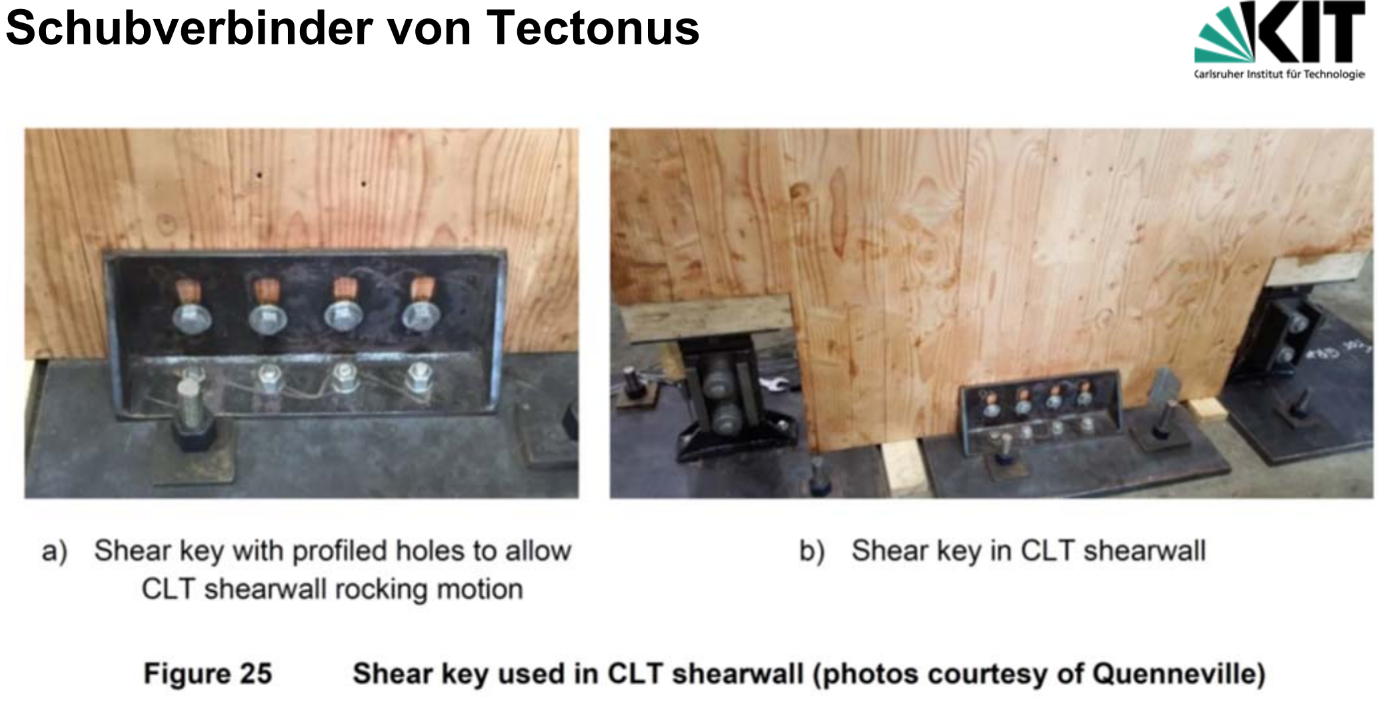
\includegraphics[width=0.45\textwidth]{Grafiken/CLT-Verbindungen/Tectonus Schubverbinder.png}\\
        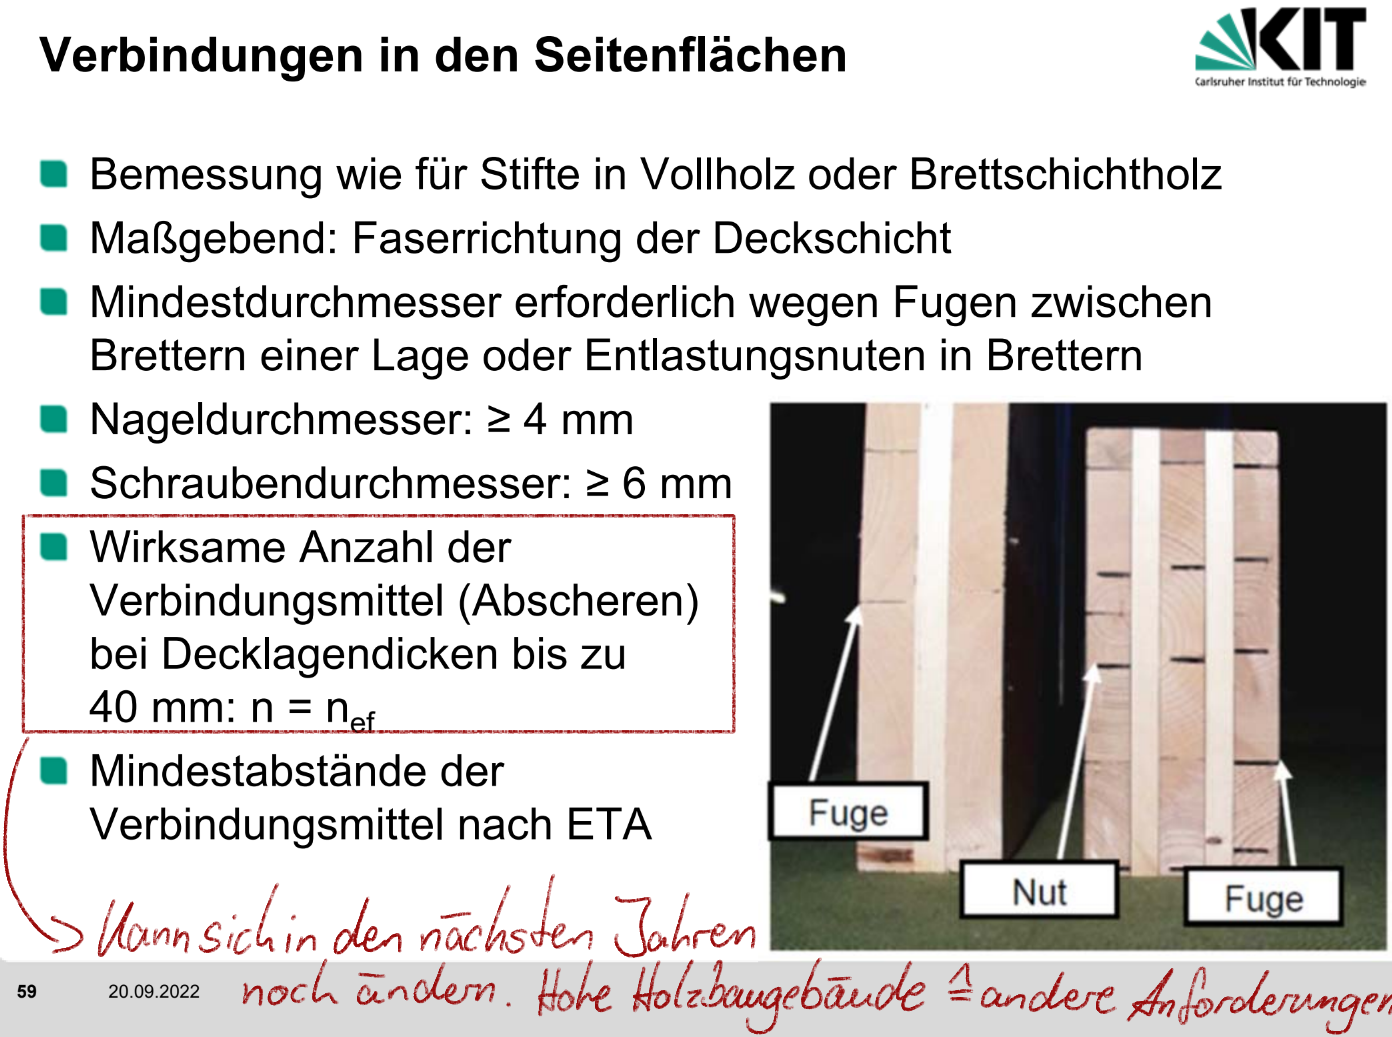
\includegraphics[width=0.45\textwidth]{Grafiken/CLT-Verbindungen/Verbindungen Seitenflächen.png}
        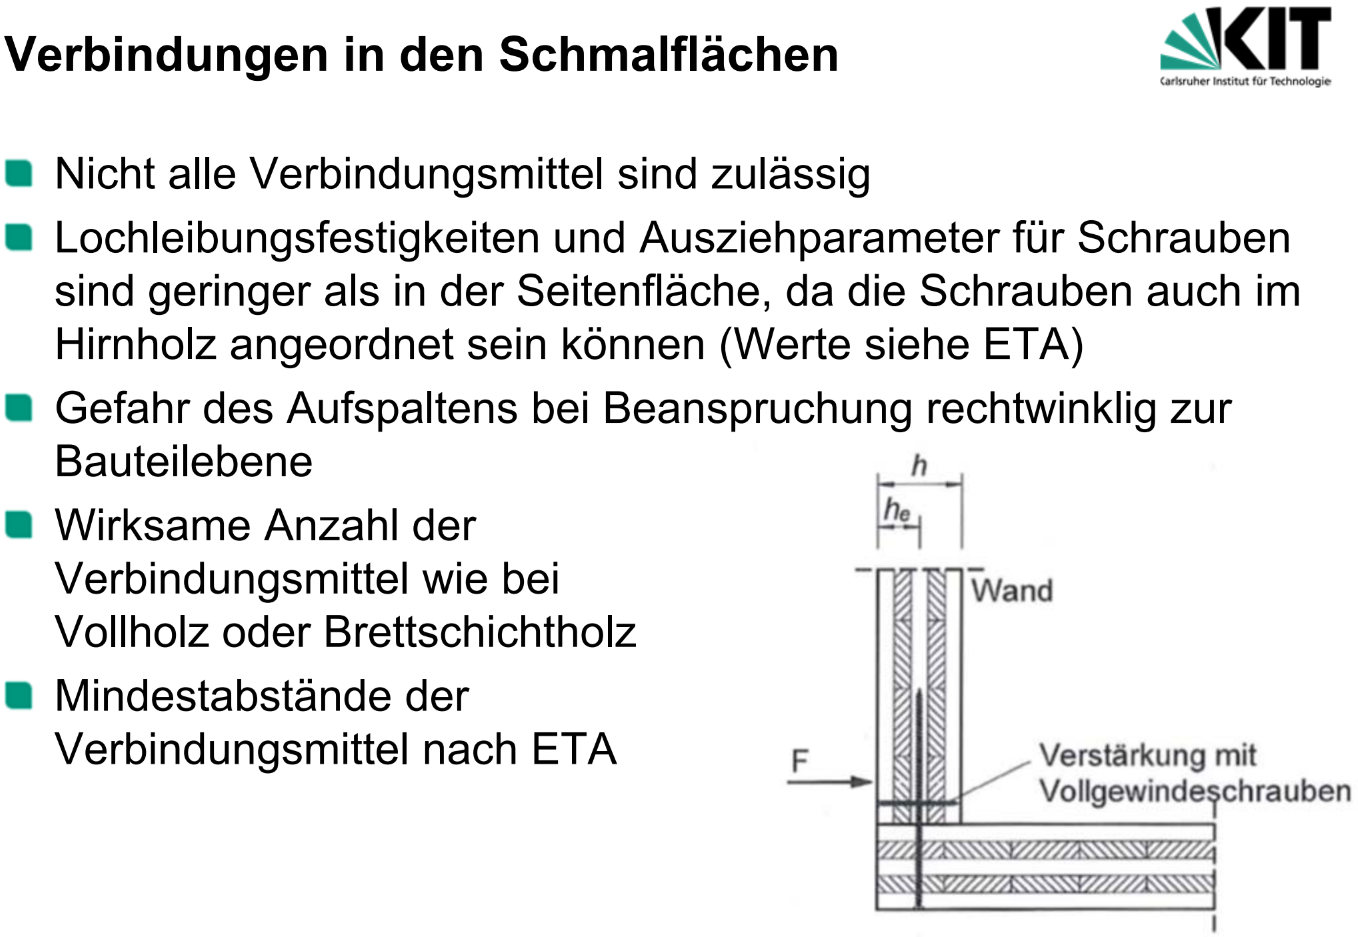
\includegraphics[width=0.45\textwidth]{Grafiken/CLT-Verbindungen/Verbindungen Schmalflaechen.png}\\
        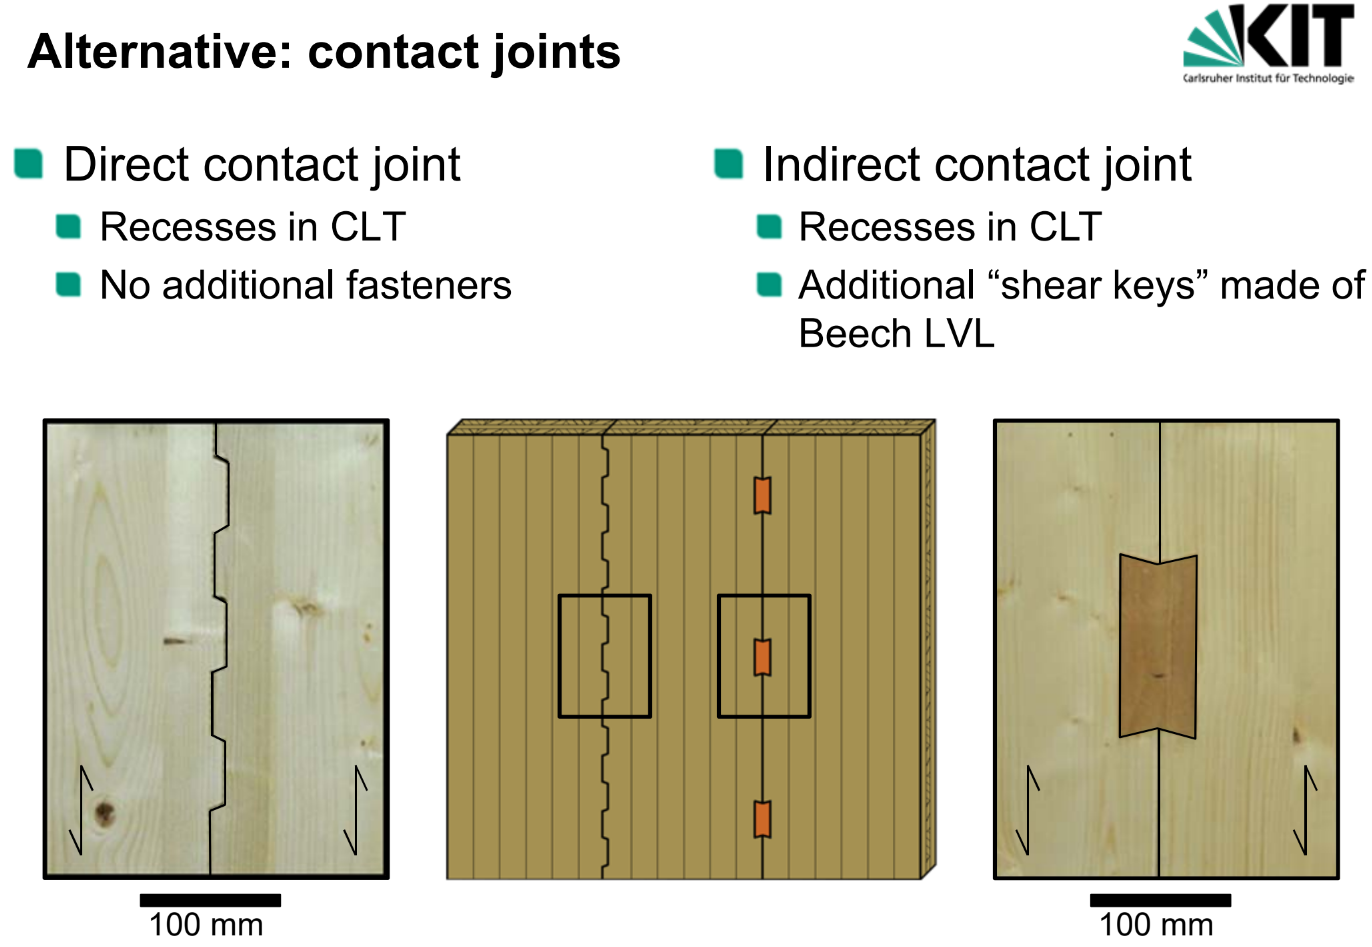
\includegraphics[width=0.45\textwidth]{Grafiken/CLT-Verbindungen/Contact joints.png}\\
        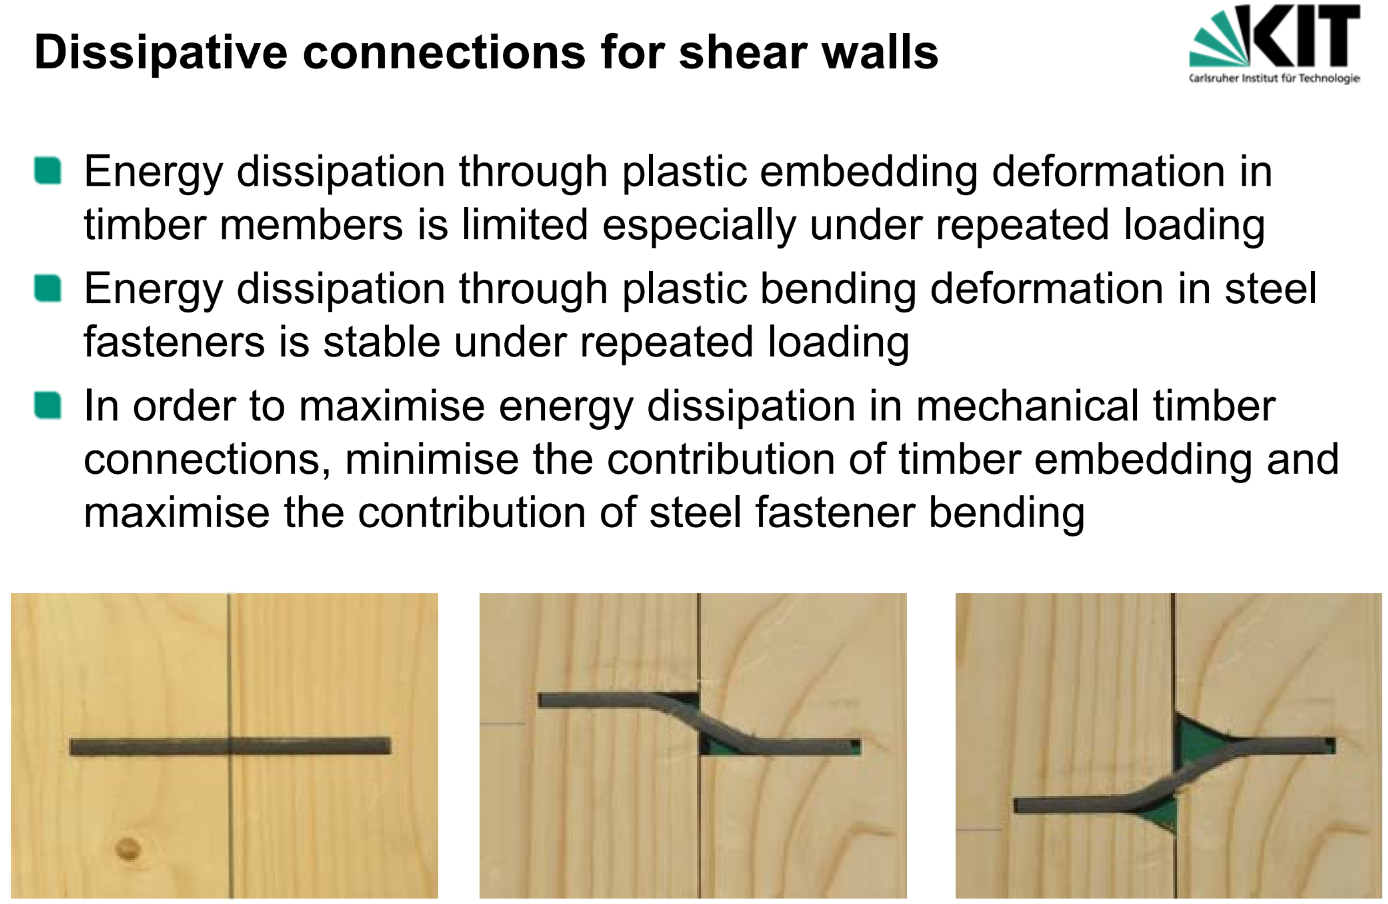
\includegraphics[width=0.45\textwidth]{Grafiken/CLT-Verbindungen/Dissipative joints.png}
        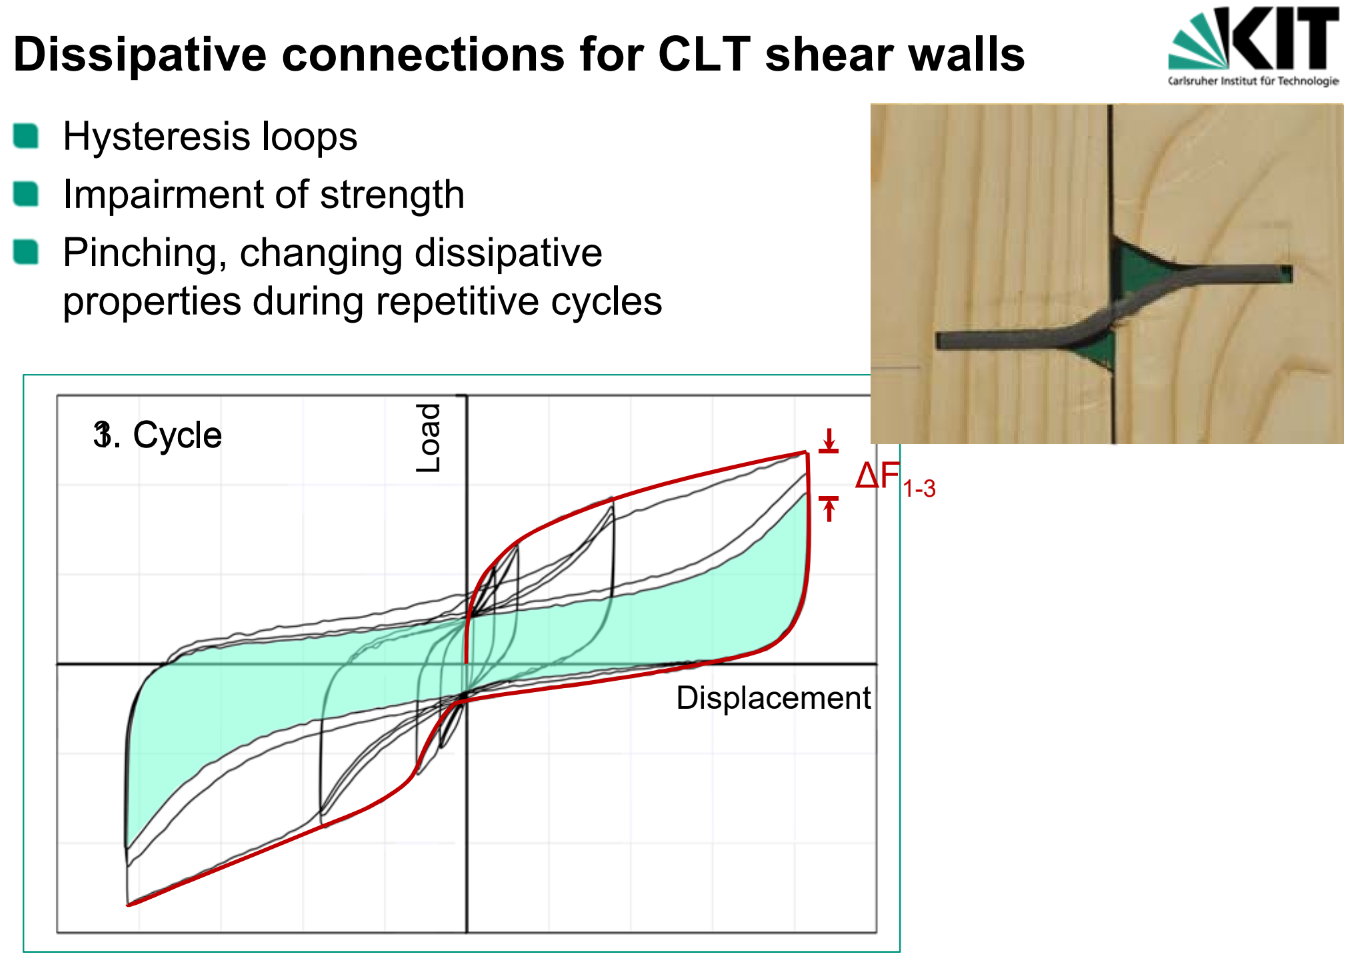
\includegraphics[width=0.45\textwidth]{Grafiken/CLT-Verbindungen/Dissipative joints hysteresis.png}\\
        
    \end{itemize}



\newpage
\section{Laubholz}

    \subsection{Häufige Vertreter:}
        \begin{itemize}
            \item Fichte (25\%)
            \item Kiefer (23\%)
            \item Buche (15\%)
            \item Eiche (10\%)
            \item Weitere: Esche, Birke, Erle, Ahorn, Pappel, Hainbuche
            \item Tendenz Laubholznutzung steigend (Fichtenwachstum rückgängig)
        \end{itemize}

    \subsection{Generelles:}
        \begin{itemize}
            \item Historische nutzung: Bauholz, Möbelbau, Schiffbau, Brennholz, Holzkohle, Teller/Besteck und Kunst (schwer zu verarbeiten, da sehr hart)
            \item Ötzi Nutzung Hartholzvarianten zu jeweiligen Stärken
            \item Aktuelle Nutzung:
                \begin{itemize}
                    \item In Zahlen:\vspace*{3mm} \\
                            \resizebox{0.9\textwidth}{!}{%
                            \begin{tabular}{|c|c|c|c|c|c|}
                            \hline
                            {[}Mio.Fm{]} & Entnahme & Sägeindustrie & Holzwerkstoffindustrie & Holzstoff/Zellstoff & Furnier-/Sperrholz \\ \hline
                            Energetische Nutzung: & 13,9 (70\%) &  &  &  &  \\ \hline
                            Stoffliche Nutzung: & 5,9 (30\%): & 2,6 (44\%) & 2,4 (40\%) & 0,7 (12\%) & 0,2 (4\%) \\ \hline
                            Gesamt: & 19,8 (100\%) & \multicolumn{1}{l|}{} & \multicolumn{1}{l|}{} & \multicolumn{1}{l|}{} & \multicolumn{1}{l|}{} \\ \hline
                            \end{tabular} } \vspace{1mm}
                    \item Schlussfolgerung:\\
                        Laubholz kann Nadelholz nicht vollständig substituieren: mangelnde Verfügbarkeit und technologische Schwierigkeiten (Verarbeitung \& Verklebung z.T. schwierig, wesentlich kürzere Standzeiten von Bearbeitungswerkzeugen, erhöhte Quellund Schwindmaße,..)\\
                        Daraus folgende Frage:
                            Wie kann Laubholz maßgeschneidert eingesetzt werden?
                                \begin{itemize}
                                    \item Höhere Rohdichte als Nadelholz $\rightarrow$ höhere Festigkeit
                                    \item Höhere Dauerhaftigkeit einiger LH-Arten:\\
                                        Robinie hat Dauerhaftigkeitsklasse 1-2 von 5 gegen Pilze\\
                                        („1 - sehr dauerhaft“ bis ${ } 5-$ nicht dauerhaft $)$
                                \end{itemize}
                \end{itemize}
        \end{itemize}

    \subsection{Relevante Holzprodukte:}
        \begin{itemize}
            \item Vollholz
            \item Brettschichtholz (BS-Holz/BSH/GLT)
            \item Brettsperrholz (BSP/CLT)
            \item Furnierschichtholz (FSH)
            \item Furniersperrholz
        \end{itemize}
    \subsection{Eigenschaften und Bemessung:}\
        \begin{itemize}
            \item Unterschiede Nadelholz - Laubholz:
                \begin{itemize}
                    \item Nadelholz ist evolutionär weniger weit entwickelt als Laubholz
                    \item Laubholz ist ausdifferenzierter in seinem anatomischen Aufbau (Nadelholz hat nur sog. „Tracheiden“ als Zelltypen)
                    \item Nadelholz ist i. a. „langfasrig" und Laubholz „kurzfasrig“
                    \item Klebeigenschaften sind z.T. anders
                    \item Bearbeitung von LH ist oft schwieriger
                    \item Laubholzprodukte i. a. teurer als Nadelholzprodukte
                \end{itemize}
            \item Links: Aufbau BaumQS Rechts: Faser-/Zellstruktur\\
                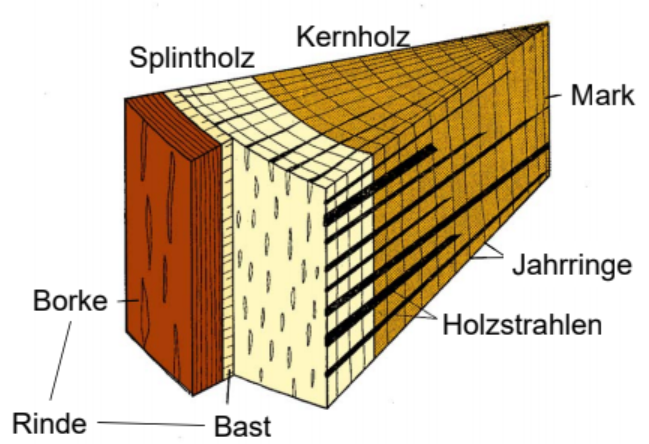
\includegraphics[width=0.45\textwidth]{Grafiken/Laubholz/BaumQS.png}
                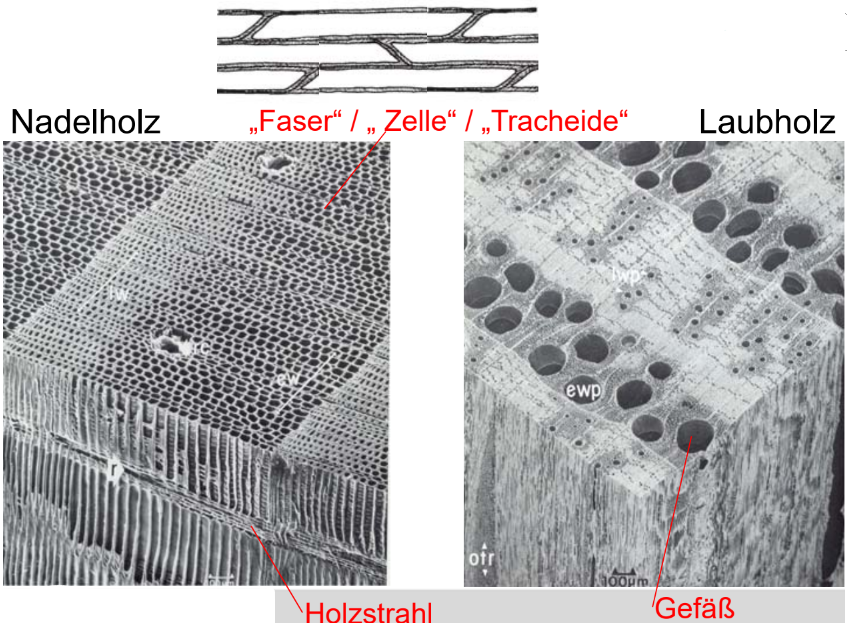
\includegraphics[width=0.45\textwidth]{Grafiken/Laubholz/Zellstruktur.png}\\
            \item Laubholzanatomie:
                \begin{itemize}
                    \item sehr vielfältig
                    \item Viele verschiedene Zelltypen:
                        \begin{itemize}
                            \item  verschiedene Tracheiden mit unterschiedlichen Funktionen:
                            z. B. „Libriformfaser" zur Festigung und
                            „Fasertracheide" zur Wasserleitung
                            \item  Gefäße zur Wasserleitung, je nach LH-Art unterschiedlich
                            \item  Parenchym zur Speicherung
                        \end{itemize}
                    \item Umwandung von Splint zu Kern ist holzartspezifisch
                        \begin{itemize}
                            \item  Einlagerung von Inhaltsstoffen mit versch. Funktionen: Farbstoffe, Gerbstoffe, Fette, Harze, Phenole, Terpene
                            \item versch. Mechanismen zum Zellabschluss, z.B. Verthyllung
                        \end{itemize}
                \end{itemize}
            \item Rohdichte und Holzfeuchte
                \begin{itemize}
                    \item LH-Arten haben wegen ihres unterschiedlichen anatomischen Aufbaus unterschiedliche Rohdichten:\\
                    Balsaholz ca. $100 \mathrm{~kg} / \mathrm{m}^3 \Longleftrightarrow$ Pockholz ca. $1200 \mathrm{~kg} / \mathrm{m}^3$
                    \item Zusätzlich bestimmen noch weitere Faktoren die Rohdichten, z.B. die Wuchsbedingungen
                    \item Holz ist hygroskopisch und seine Eigenschaften sind bis zum Fasersättigungsbereich feuchteabhängig
                    \item Holzfeuchteänderungen unterhalb des Fasersättigungsbereichs führen zu Schwind- und Quellverformungen
                    \item Schwindverformungen tangential sind am größten
                \end{itemize}
                    $\Rightarrow$ Betrachtung auf Holzartebene bei LH wichtiger als bei NH
            \item Eigenschaften und Verwendung:
                \begin{itemize}
                    \item Hainbuche/Weißbuche:
                        \begin{itemize}
                            \item Hohes Schwindmaß
                            \item Verwendung: WerkzeugbaU, Klavierbau
                            \item Nicht relevant für Bauwesen durch geringe Dauerhaftigkeit
                        \end{itemize}
                    \item Pappel:
                        \begin{itemize}
                            \item Nicht dauerhaft
                            \item Verwendung: Papierindustrie
                            \item Bauwesen: Holzwerkstoffplatten, BS-Holz
                        \end{itemize}
                    \item Bergahorn:
                        \begin{itemize}
                            \item Nicht dauerhaft
                            \item Verwendung: Möbel, Parkett
                            \item Nicht relevant für Bauwesen durch geringe Dauerhaftigkeit
                        \end{itemize}
                    \item Schwarzerle:
                        \begin{itemize}
                            \item Nur unter Wasser dauerhaft
                            \item Nicht relevant für Bauwesen
                        \end{itemize}
                    \item Robinie:
                        \begin{itemize}
                            \item Sehr dauerhaftes Holz
                            \item Verwendung: Spielplätze
                            \item Bauwesen: Rundholz oder BS-Holz
                        \end{itemize}
                    \item Esche:
                        \begin{itemize}
                            \item Nicht dauerhaft
                            \item Hartes und elastisches Holz
                            \item Verwendung: Wekzeug, Möbel Parkett, Thermoholz
                            \item Bauwesen: BS-Holz, BSP, FSH
                        \end{itemize}
                    \item Gemeine Birke:
                        \begin{itemize}
                            \item Nicht dauerhaft
                            \item Stört Abbinden von Zement
                            \item Verwendung: Sperrholz
                            \item Bauwesen: Sperrholz, BS-Holz, BSP, FSH
                        \end{itemize}
                    \item Edelkastanie:
                        \begin{itemize}
                            \item Dauerhaft
                            \item Bauwesen: BS-Holz
                        \end{itemize}
                    \item Stieleiche:
                        \begin{itemize}
                            \item Wenig bis Dauerhaft
                            \item Reich an Gerbsäure
                            \item Verwendung: Bauwesen, Möbel, Parkett, Innenausbau
                            \item Bauwesen: BS-Holz, BSP
                        \end{itemize}
                    \item Rotbuche:
                        \begin{itemize}
                            \item Nicht dauerhaft
                            \item Verwendung: Sperrholz, Möbelbau, Werkzeugindustrie
                            \item Bauwesen: Sperrholz, BS-Holz, BSP, FSH
                        \end{itemize}
                \end{itemize}
                Übersicht: \vspace*{3mm}\\
                    $\begin{array}{|c|c|c|c|c|}
                        \hline \text { Holzart } & \begin{array}{c}
                        \text { Rohdichte in } k g / m^3 \\
                        \text { (bei ca. 12\% ~ )} 
                        \end{array} & \begin{array}{c}
                        \text { Schwindmaß } \\
                        \text { radial }
                        \end{array} & \begin{array}{c}
                        \text { Schwindmaß } \\
                        \text { tangential }
                        \end{array} & \text { Dauerhaft } \\
                        \hline \text { Fichte } & 330 \ldots 470 \ldots 680 & 0,17 \% & 0,32 \% & \text { nein } \\
                        \hline \text { Pappel } & 400 \ldots 450 \ldots 560 & 0,16 \% & 0,28 \% & \text { nein } \\
                        \hline \text { Robinie } & 720 \ldots 790 \ldots 950 & 0,23 \% & 0,35 \% & \text { ja } \\
                        \hline \text { Esche } & 450 \ldots 690 \ldots 860 & 0,19 \% & 0,33 \% & \text { nein } \\
                        \hline \text { Birke } & 510 \ldots 650 \ldots 830 & 0,21 \% & 0,29 \% & \text { nein } \\
                        \hline \text { Eßkastanie } & 590 \ldots 620 \ldots 660 & 0,15 \% & 0,24 \% & \text { ja } \\
                        \hline \text { Eiche } & 430 \ldots 690 \ldots 960 & 0,19 \% & 0,32 \% & \text { ja - jein } \\
                        \hline \text { Buche } & 540 \ldots 720 \ldots 910 & 0,21 \% & 0,41 \% & \text { nein } \\
                        \hline
                    \end{array}$

                \item Bemessung:
                    \begin{itemize}
                        \item Baubuche: 
                            \begin{itemize}
                                \item NKL 3 auf gar keinen Fall, sehr feuchtempfindlich, geht auch nicht mehr ganz zurück
                                \item Problematik mit Richtugnsabhängig komplizierter Bemessung durch Schichtenaufbau
                                \item Brettsperrholz vs Brettstapelholz \\
                                    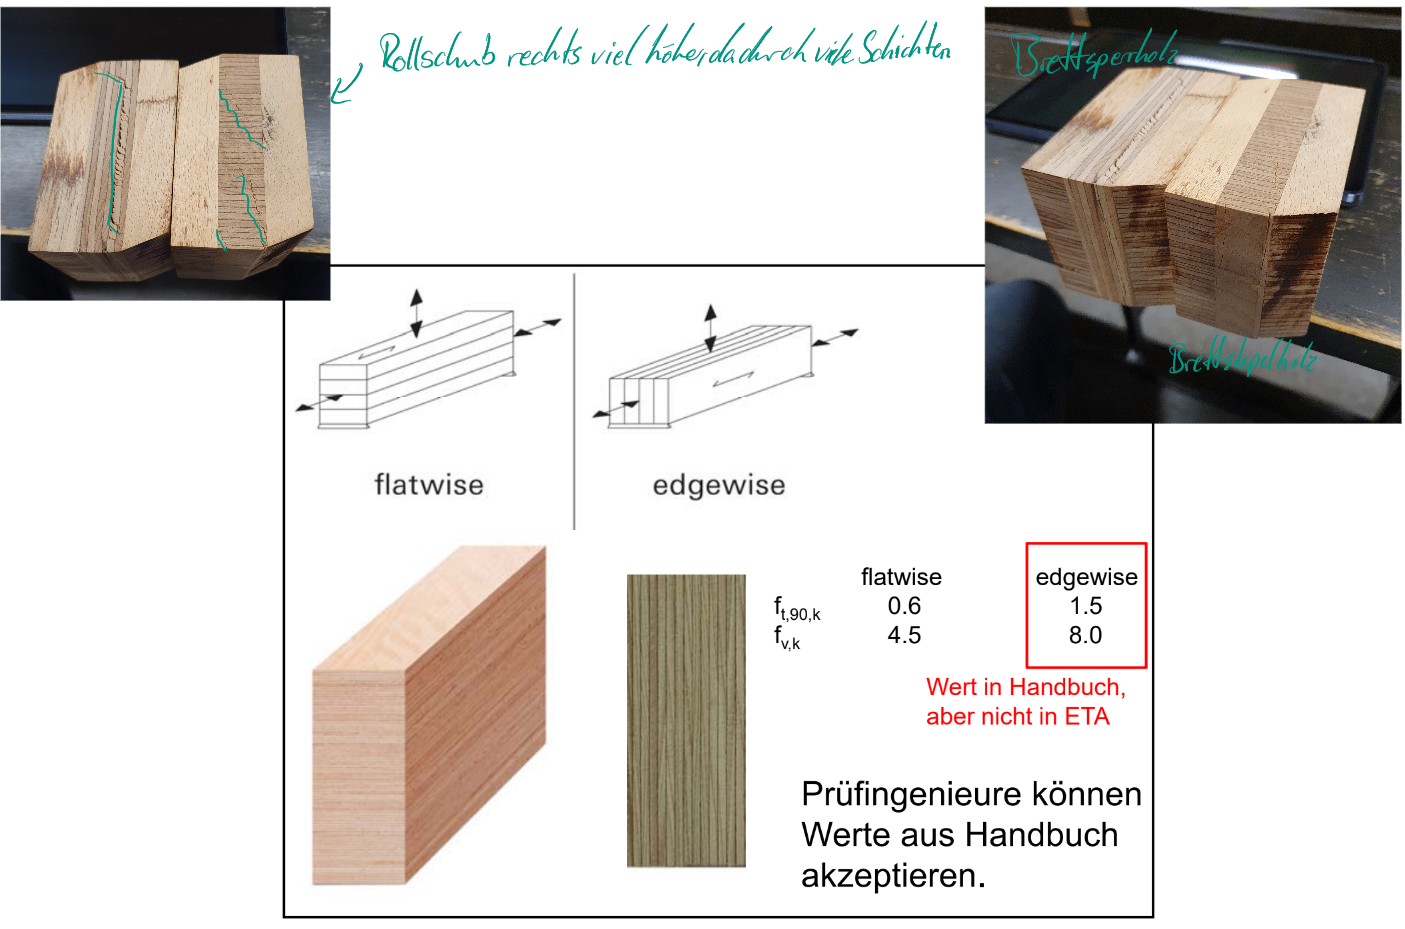
\includegraphics[width=0.45\textwidth]{Grafiken/Laubholz/Baubuche Brettsperr-Brettstapel.png}
                            \end{itemize}
                        \item Ausnutzen hoher Festigkeiten schwierig, da andere versagen vorher eintreten. Lösungen:
                            \begin{itemize}
                                \item Aufgelöste Tragwerke (Fachwerk)
                                \item Hybride Produkte (kombiniertes BS-Holz, Furnier in Zug-/Druckzone, homogenes Holz)
                                \item Lokale Verstärkungen
                                \item Ausnutzung der hohen Druckfestigkeiten
                            \end{itemize}
                    \end{itemize}
        \end{itemize}
\newpage
\section{Laubholzverbindungen}


\newpage
\section{Holzfeuchte}


\newpage
\section{Erdbeben}


\subsection{Kettenbindung}

%\begin{center} \includegraphics[width=0.55\textwidth]{Grafiken/Geschichte des Holzbaus/Kettenbindungen.png} \end{center}

\subsection{Geschoss- bzw. Ständerbau}
    \begin{minipage}{0.6\textwidth}
    \begin{itemize}
        \item 
    \end{itemize}
    \end{minipage}
    \begin{minipage}{0.4\textwidth}
       % \includegraphics[width=0.9\textwidth]{Grafiken/Geschichte des Holzbaus/Geschoss- bzw. Staenderbau.png}
    \end{minipage}
    
    
\subsection{Stockwerksbau}


\section{Klausurfragen}

    \begin{itemize}
        \item Wie werden Holztafeln miteinander verbunden?
    \end{itemize}
 
 
 
 
\end{document}